\chapter{Design and Implementation of the G1 Family of Garbage Collectors}
\label{cha:implementation}

As briefly discussed in the previous chapter, the four well-known region-based collectors, Garbage-First GC, Shenandoah GC, C4 GC, and
ZGC share many common design parts such as concurrent marking algorithm, region-based
structure and allocation algorithm. However, there are also several differences
among them, especially the different techniques designed to improve GC performance.
Hence their resulting GC performances are different.

As a major contribution of this thesis, this chapter explores the underlying relationships
among these collectors, which the original designers of these GCs were not aware of.
Based on these discovered connections, this chapter also discusses the implementations
of several region-based GCs, which I called "The Garbage-First family of garbage collectors",
as a series of improvements inferred by the relationships.

Section~\ref{sec:generaldesign} describes the general and high-level design of the
G1 family of garbage collectors and explores their underlying relationships.
Section~\ref{sec:simpleregiongc} describes the implementation details of a simple region-based GC.
Section~\ref{sec:linearscangc} describes the implementation of the simple region-based GC that uses linear scanning for evacuation.
Section~\ref{sec:concmarkgc} describes the implementation of the concurrent marking algorithm.
Section~\ref{sec:g1gc} describes the details of implementing the Garbage-First GC
Section~\ref{sec:shenandoahgc} describes the details of implementing the Shenandoah GC



\section{General Design}
\label{sec:generaldesign}

The general design of the implementation including reconsidering the underlying
relationship among all the existing region-based garbage collectors, reordering them
and implementing them to reflect such relationships.

\subsection{Analysis of the collectors and their relationships}

The four well-known region-based garbage collectors, G1 GC, Shenandoah GC, C4 GC, and
ZGC share plenty of common design and algorithms. The major similarity of these collectors
is that they are pauseless collectors designed for modern Java Virtual
Machines and attempt to improve GC performance when targeting large heaps.

The same design goal leads to the similar general structure of these collectors.
As described in publications by \cite{detlefs2004garbage}, \cite{flood2016shenandoah},
\cite{tene2011c4} and \cite{liden_karlsson_2018}, their similarities include:

\begin{quote}
  \textbf{Region-based memory structure}
    which divides the whole heap up into smaller regions and performs collection
    on a subset of regions during each GC (such subset is called the "collection set").

  \textbf{Bump pointer allocator}
    which uses an allocation algorithm that linearly allocates objects within the memory
    slice of a region and moves to another available region when the current region is filled.

  \textbf{Concurrent marking}.
    At the beginning of each GC cycle, all of the collectors use the Snapshot-at-the-beginning algorithm
    (firstly introduced by \cite{yuasa1990real}) to mark all live objects in the heap
    concurrently without stopping the mutators.

  \textbf{Perform heap defragmentation}
    after the marking phase, including copying live objects in the collection set to other
    regions before releasing the memory in the collection set.
\end{quote}

Differences also exist among these collectors. These garbage collectors adopt
different techniques to reduce the GC pause time and increase the mutator throughput.
Specifically,

\begin{quote}
  Garbage-first GC uses a data structure called "remembered set" to record the
  cross region pointers during the execution of the Java program.
  Later during evacuation phase, instead of walking over the whole object graph to update
  references as what other collectors (e.g. SemiSpace GC) did, G1 only needs to scan the
  remembered sets to update cross region pointers pointing to the collection set.
  Also, G1 has a generational mode which eagerly collects newly allocated objects
  during nursery GCs.

  Shenandoah GC performs the evacuation phase concurrently, by using the
  Brooks indirection barrier (which was first introduced by \cite{brooks1984trading}).
  Although Shenandoah GC still performs full heap tracing during the evacuation phase,
  the GC pause time is extremely low and is not proportional to the heap size.

  ZGC can be simply regarded as an improvement over the Shenandoah GC with high mutator performance.
  ZGC uses the "colored pointers"
  as well as a highly optimized read barrier to assist with the Brooks indirection barrier
  to further increase the mutator throughput.

  C4 GC is very similar to ZGC and also performs concurrent evacuation during each
  GC. The major difference to ZGC is that C4 GC is generational which is expected
  to have higher performance than ZGC.
\end{quote}

In general, these four collectors are strongly related to each other in terms of
the design and algorithm structure. In addition, each collector performs their
own enhancements to improve GC performance. In this way, at the algorithmic level,
these collectors tend to be a set of improvements over the naive region-based collector.
Hence they are more likely to form as a family of collectors
instead of individual and unrelated collectors.

\subsection{Implementation steps}

As the first implementation which reflects such algorithmic hierarchy,
members of the G1 family of garbage collectors are reorganized and reimplemented on JikesRVM
by following different steps against the original implementations. 

I started from implementing a simple region-based GC which divides the whole Java heap
up into fix sized regions. During each GC cycle it performs fully stop-the-world but parallel object marking
and full-heap tracing based object evacuation.
Then I made progressive improvements based on this collector to further implement some G1 family of garbage collectors.

Since both Garbage-first and Shenandoah GC use heap linear scanning for evacuation,
I implemented a linear-scan region-based GC by dividing the heap evacuation phase
of the simple region-based GC into two phases: The linear scan evacuation phase
and the reference updating phase.

Then I changed the stop-the-world marking phase of the linear-scan region-based GC
to the concurrent marking phase to implement a concurrent-marking region-based GC.
The Snapshot at the Beginning algorithm (\cite{yuasa1990real}) was used to implement the concurrent marking phase.

By adding the remembered-sets to the concurrent-marking region-based GC
and switching to remembered-set based evacuation,
I implemented the Garbage-first collector.

Also, starting from the concurrent-marking region-based GC, by implementing the Brooks indirection pointers
and the corresponding mutator barriers, I implemented the Shenandoah GC.

By performing such progressive improvements, I successfully implemented a series of
G1 family of garbage collectors and share as much code and design as possible
among the implementations of these collectors. Which enables the possibility for future
algorithmic-level analysis on these garbage collectors. The other two discussed
collectors, C4 GC and ZGC, are not implemented and evaluated in this project.

\section{Simple Region-based GC}
\label{sec:simpleregiongc}

This simple region-based GC is provided as a baseline for future implementation of the G1 family of collectors.
It contains most basic structures of the Garbage-first family of garbage collectors such as
the region-based heap space and bump pointer allocation algorithm. By making progressive improvements
over this region-based GC, I keep the implementation differences among the
G1 family of garbage collectors to a minimum.

\subsection{Heap structure and allocation policy}

This simple region-based GC and other GCs discussed later all use the same implementation of the
heap structure (which is implemented in \textjava{RegionSpace} and \textjava{Region} classes) and the
same allocation policy (which is implemented in the \textjava{RegionAllocator} class).
The \textjava{RegionSpace} divides the whole heap up into fixed 1\,MB regions, which
are 256 MMTk pages.

Figure~\ref{fig:allocator} shows the code for allocation objects within the region space.
To allocate objects, for each allocator, it firstly requests a region of memory (256 pages) from the page resource.
Then it makes the allocation cursor points to the start of the region and bump increase this
allocation cursor to allocate objects. Figure~\ref{fig:allocator:fast} shows the code for such
allocation fast path. Most of the object allocation processes will only follow the
fast path. 
After a region is filled, to allocate a new object, the mutator enters a slow path
which is shown in figure~\ref{fig:allocator:slow}.
In this slow path the allocator moves the bump pointer to another newly acquired region for future allocations.

MMTk reserves some extra pages for each region to record metadata.
After the allocator filled a region, it records the end address of the region in the metadata pages for 
region linear scanning which is lately used in some collectors. Also, an off-heap bitmap is
maintained in the region's metadata pages to record the liveness data of objects in this region.

\begin{figure}
  \centering
  \begin{subfigure}[a]{\textwidth}
    \lstinputlisting[linewidth=\textwidth,breaklines=true]{code/alloc-fast.java}
    \caption{Region allocator - fast path}
    \label{fig:allocator:fast}
  \end{subfigure}

  \begin{subfigure}[b]{\textwidth}
    \lstinputlisting[linewidth=\textwidth,breaklines=true]{code/alloc-slow.java}
    \caption{Region allocator - slow path}
    \label{fig:allocator:slow}
  \end{subfigure}

  \caption{Region Allocator}
  \label{fig:allocator}
\end{figure}

\subsection{Stop-the-world marking}

Based on the high-level design of MMTk, after each allocation MMTk checks if a stop-the-world
or concurrent GC is required for the currently selected GC plan.
For this simple region-based GC, only stop-the-world collections are triggered.

The region-based GC initiates a collection cycle when the free heap size is less than
the pre-defined \textjava{reversedPercent} (default is 10\%). During each GC cycle,
the collector starts by performing a full heap tracing to recursively mark all live objects.
The marking algorithm considers the heap as a graph of objects and follows the idea of breadth-first graph search
which firstly scans and marks all the stack and global root objects and pushes them into an object queue.
Then the collector threads keep popping objects from the object queue and collecting all its
object reference fields (which are child nodes of the current object node in the object graph).
If these object fields were not marked previously, the collector then marks and pushes them back into the object queue.
The marking process is done when all of the local and global object queues are drained, which means all objects that are reachable
from the root objects are marked after the marking phase.

Instead of using the GC byte in the object header for marking which is widely used in other GCs in MMTk,
a bitmap for each region is maintained to record the liveness data of the objects.
At the start of the marking phase, bitmaps of all regions are initialized to zero.
As shown in figure~\ref{fig:tracemarkobject}, during visiting each object, the collector attempts to set the mark bit
of the current object in the bitmap and push the object into the object queue only if the attempt operation succeeds.

Although using such extra "liveness table" is not necessary for this region-based GC,
this is a common design for Garbage-first and Shenandoah GC.
So the GC byte in the object header was disabled at the very beginning to reduce the implementation difference among all the collectors.

\begin{figure}
  \centering
  \lstinputlisting[linewidth=\textwidth,breaklines=true]{code/tracemarkobject.java}
  \caption{Code for mark each object}
  \label{fig:tracemarkobject}
\end{figure}

\subsection{Collection set selection}

As shown in figure~\ref{fig:tracemarkobject}, during the processing of each object in the heap,
the collectors also atomically increase the live bytes for each region, starting from zero.
After the full heap marking phase, the collector starts a collection set selection phase to construct
a set of regions for later defragmentation.

The collection set selection phase firstly takes a list of all allocated regions,
sort them in ascending order by the live bytes of the region.
Then the collector selects the regions with lowest live bytes.
Also, the collector should make sure the total count of live bytes in the collection set is not
greater than the free memory size of the heap, to prevent the to-space from being exhausted during evacuation.

At the end of the collection set selection phase, the collector marks all regions
in the collection set as "\textjava{RELOCATION_REQUIRED}" for the future evacuation phase.

\subsection{Stop-the-world evacuation}

The evacuation phase is a fundamental part of the copying collectors.
It tries to avoid heap fragmentation by forwarding the live objects in highly fragmented memory slices
and moving them together.

For this simple region-based GC, the evacuation phase is performed after the end of the collection set selection phase.
This evacuation phase is aimed to copy/evacuate all live objects in the collection set to other
regions.

Figure~\ref{fig:traceevacuateobject} shows the process of evacuating an object.
To evacuate objects, the collector performs another full heap tracing to remark all the objects,
just like the marking phase discussed before.
But in addition to marking the objects, the collector also copies the objects and atomically update the forwarding status in the object header
if the object is in the collection set.
Such full heap tracing ensures all objects that were marked in the marking phase are also being scanned and remarked in the evacuation phase.
Which means that all live objects in the collection set are processed and evacuated properly.

At the end of the evacuation phase, after all objects are evacuated, the whole stop-the-world GC cycle is finished.
The collector frees all the regions in the collection set and resumes the execution of all the mutators.

\begin{figure}
  \centering
  \lstinputlisting[linewidth=\textwidth,breaklines=true]{code/traceevacuateobject.java}
  \caption{Code for evacuate each object}
  \label{fig:traceevacuateobject}
\end{figure}

\subsection{Evacuation correctness verification}

Since the region-based evacuation is a fundamental component of the G1 family of garbage collectors
and can have several variants (e.g. concurrent evacuation), it is necessary to verify the correctness of the evacuation process.
I used an additional full heap tracing for verification. The full heap tracing is
similar to the marking trace and is fully stop the world to ensure the object graph is never changed
during the verification process.
When visiting each object node during verification, the collector checks all its object reference fields
and ensure they are either null or pointing to the valid Java objects.
The collector also checks no object node should be located in the from space (i.e. the collection set).

This full heap tracing verification process is optional and can be switched on and off for
debugging purposes.
At the end of the verification process, we can assert that the whole Java heap is
not broken and is in the correct status.

\section{Linear Scan Evacuation}
\label{sec:linearscangc}

Since both Garbage-First and Shenandoah GC use heap linear scanning for evacuation,
I implemented a linear-scan evacuation version of the simple region-based GC.

In the simple region-based GC, both object evacuation and reference updating are
done together during the stop-the-world evacuation phase, by using a single full heap tracing.
For this linear-scan region-based GC, I split the stop-the-world evacuation phase into
two phases: The linear scan evacuation phase and the reference updating phase.

During the linear scan evacuation phase, the collector threads linear scan all the regions
in the collection set and evacuate live objects in these regions. The collector does not
fix or update any references during this phase.

During the reference updating phase, the collector performs a full-heap tracing,
just likes the evacuation phase of the simple region-based GC, but only fixes and updates
pointers to ensure every pointer in the heap points to the correct copy of the object.

By separating the linear scan evacuation phase and the reference updating phase,
the linear-scan region-based GC reveals the basic collection processes of most G1 family
of garbage collectors: \textjava{marking -> evacuation -> update references -> cleanup}.
The modular design of this collectors enables the future redesign and rewrite of some specific
phases, e.g. concurrent marking, remembered-set based evacuation or concurrent evacuation.

\section{Concurrent Marking}
\label{sec:concmarkgc}

Another improvement I did is to make the marking phase concurrent to reduce the
mutator latency caused by the stop-the-world object marking.
This concurrent-marking region-based GC is an improvement over the previous linear-scan region-based GC.

The concurrent marking phase uses the Snapshot-at-the-beginning (SATB) algorithm.
This algorithm was first introduced by \cite{yuasa1990real} to
complete most of the marking work concurrently without pausing mutators.
The SATB algorithm assumes an object is live if it was reachable (from the roots)
at the start of the concurrent marking or if it was created during the concurrent markin.

The whole marking phase consists of two pauses: the initial mark pause and final mark pause.
During the initial mark pause, same as the stop-the-world marking phase,
the collector clears the live bitmap for all regions,
and then it scans and process all the root objects including stack objects and global objects.
After that, the collector resumes all the mutators and concurrently marks all the remaining object.
If the mutators allocate spaces too quick and the used ratio of the heap reaches
the stop-the-world GC threshold previously defined in the simple region-based GC, the
collector then pauses all the mutators and switches to a stop-the-world marking phase
to continue the marking process.

\subsection{SATB write barriers}

As part of the SATB algorithm, to maintain the invariant of "An object is live if it was live at the start of marking",
the mutators in this concurrent-marking GC implemented a SATB barrier, which is a piece of code
fragment inserted into the java program, before every object field write, object field compare \& swap
and object array copy operations in the program.
Figure~\ref{fig:satbbarrier} shows the object reference write barrier that is used
to track every object graph modifications during the concurrent marking.
When an object reference field modification happens, since the old child object reference
was reachable from the roots before this modification, it should be considered as a live object.
So the SATB barrier traces and enqueues this old object reference field to ensure it is marked as live.
Same as the stop-the-world marking process, the concurrent marking phase finishes after
the local and global object queues are drained.

During the final mark pause, the collector releases and resets the marking buffer that
was used for concurrent marking. Then it starts the collection set selection phase, just like the
simple region-based GC.

This concurrent-marking region-based GC is an important enhancement which enables
the analysis of the pause time and mutator latency due to the SATB concurrent marking algorithm on the region space.
Although MMTk provides an implementation of SATB algorithm, the old implementation
is only performed on the mark-sweep space, not on the region space.
By analyzing this implementation of the concurrent-marking algorithm,
it is able to understand the detailed performance impact of the Garbage-first and Shenandoah GC due to the SATB algorithm.

\begin{figure}
  \centering
  \begin{subfigure}[a]{\textwidth}
    \lstinputlisting[linewidth=\textwidth,breaklines=true]{code/satb-barrier.java}
    \caption{The SATB Barrier which enqueues objects into a SATB buffer}
    \label{fig:satb:enqueue}
  \end{subfigure}

  \begin{subfigure}[b]{\textwidth}
    \lstinputlisting[linewidth=\textwidth,breaklines=true]{code/satb-object-field-write.java}
    \caption{SATB mutator barriers}
    \label{fig:satb:ofw}
  \end{subfigure}

  \caption{Snapshot at the Beginning Barriers}
  \label{fig:satbbarrier}
\end{figure}

\section{Garbage-First GC}
\label{sec:g1gc}

Garbage-First (G1) GC (\cite{detlefs2004garbage}) was originally designed by Oracle to replace
the old Concurrent Mark and Sweep GC. G1 GC was designed to target large heap but
has a reasonable and predictable GC pause time. To achieve a short pause time, G1
uses a data structure called remembered-set to perform partial heap scanning during the
pointer updating phase, instead of performing a the full-heap scanning. To make the GC time predictable,
a pause time prediction model is involved in G1 to predict and choose the number regions in the
collection set to meet a soft real-time pause goal. In addition, G1 has a generational
mode which performs nursery GCs that collects young (newly allocated) regions only.

During each GC cycle of G1 GC, there are 5 major phases.
The first three phases are the concurrent marking phase, the collection
set selection phase and the linear scan evacuation phase,
same as the concurrent-marking region-based GC.
The fourth phase is the remembered-set based pointer updating phase.
And the last phase is the cleanup phase which frees the regions in the collection set.

The construction of the Garbage-first GC on JikesRVM is based on the concurrent-marking
region-based GC.
It involves three improvements over the concurrent region-based collector discussed in Section~\ref{sec:concmarkgc}:
remembered-set based pointer updating, pause time predictor and generational collection.
The remembered-set based pointer updating phase largely reduces the pause time by
avoiding full heap tracing when performing reference updating, by using remembered sets.
The pause time predictor uses a statistical prediction model to make the pause time of each
GC more predictable and not exceeds a soft pause time goal.
The generational mode enables G1 to collect garbage more efficiently by collecting young objects earlier.
% Under the help of the generation assumption of objects, which under most cases
% further reduces the average pause time of GCs

\subsection{Remembered-set}

Under the G1 collection policy, the region space further divides regions into fixed 256\,B cards for constructing remembered sets.

Figure~\ref{fig:remset} shows the general structure of a remembered-set.
The remembered-set is a data structure for each region to remember cross
region pointers in other regions that pointing to objects in the current region.
A remembered-set for a region is implemented as a list of PerRegionTables.
A PerRegionTable in the remembered-set is a bitmap corresponds to a region in the heap.
The bitmap records cards in the corresponding region that contains pointers pointing to the
current region. Each bit in the bitmap corresponds to one card.

\begin{figure*}
  \centering
  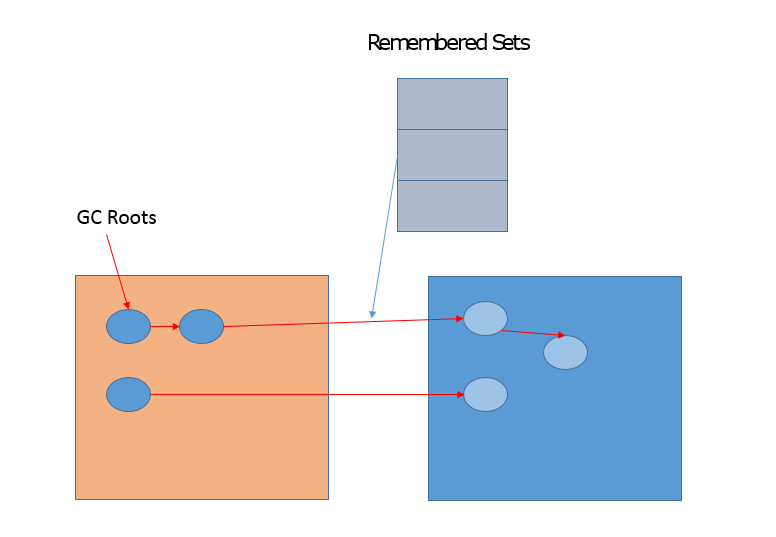
\includegraphics[width=\textwidth/2]{{figs/remset.png}}
  \caption{Remembered-Set Structure}
  \label{fig:remset}
\end{figure*}

The remembered-sets are maintained by the collector and should be updated
at every object field modification operation to ensure the correctness of the remembered-sets.

\subsection{Concurrent remset refinements}

As shown in figure~\ref{fig:remsetbarrier}, in order to maintain the structure of remembered-sets,
a new barrier called "remembered-set barrier" was involved for each object field modification action in the Java program.
For each object field modification \textjava{obj.x = y}, the remembered-set barrier checks
whether the pointer \textjava{y} is a cross region pointer (i.e. not pointing to the region that contains \textjava{obj}).
If the check succeeds, the remembered-set barrier enters a slow path which marks the
card containing \textjava{obj} and pushes this card into a local \textjava{dirtyCardBuffer}.
Since the minimum memory allocation unit in the MMTk metadata space is one page (4\,KB), the size of
the local \textjava{dirtyCardBuffer} is 1024 cards, instead of 256 cards which are used by the original G1 design.

\begin{figure}
  \centering
  \lstinputlisting[linewidth=\textwidth,breaklines=true]{code/remsetbarrier.java}
  \caption{Remembered-set Barrier}
  \label{fig:remsetbarrier}
\end{figure}

When the local \textjava{dirtyCardBuffer} is full, the remembered-set barrier
pushes the local \textjava{dirtyCardBuffer} to the global filled RS buffer set.
And when the size of the global filled RS buffer set reaches a threshold of 5 \textjava{dirtyCardBuffer}s,
a concurrent remset refinement is triggered.
A separate concurrent remset refinement thread was started to process each
\textjava{dirtyCardBuffer} in the global filled RS buffer set.
The refinement thread scans each card of each \textjava{dirtyCardBuffer}.
If the card is marked, then clear its marking data, linear scan it for cross-region pointers
and updates the corresponding remembered-set for each cross-region pointer.

\subsubsection{The card table}

To perform card marking and card linear scanning during concurrent remset refinements,
A card table should be used to record the marking data for each card as well as the offset
of the first and the last object for each card.
The card table consists of three parts. a) A bitmap of all cards in the Java heap
to record the marking data of the cards. b) A byte array (i.e. a byte map) to record the
offset of the first object for each card. c) Another byte array to record the
offset of the last object for each card.

\subsubsection{Hot cards optimization}

During concurrent remset refinements, some cards may be enqueued and scanned multiple times.
This can cause extra computation costs. To avoid such redundant scanning,
a hotness value is assigned for each card. Every scan on a card increases its hotness value by 1.
When the hotness value for a card exceeds a threshold (default is 4), this card is considered
as a "hot card". Hot cards are pushed into a separate hot cards queue and the processing
of all the hot cards card is delayed until the start of the evacuation phase.

\subsection{Evacuation phase}

G1 uses linear scan evacuation, just like the beforehand discussed collectors.
During the evacuation phase, the collector linear scans each region in the collection
set and copy live objects to the to-regions.

\subsection{Remembered set based pointer updating}

By performing concurrent remset refinements, G1 GC can ensure that the structure of all remembered-sets is always maintained correctly.
Which enables the partial heap scanning for pointer updating, without a full heap tracing.

After the collection set selection phase, the collector firstly performs a linear
scan over regions in the collection set to evacuate all live objects in the collection set.
Then the collector starts a references updating phase which considers
the root set as the union of all root objects and objects in the cards that are recorded in the remembered-sets.
During references updating phase, instead of performing a full heap tracing to fix and
update all the references in the heap, the collector only scans root objects and
cards in remembered-sets to update references,
because all pointers that need to be updated are either root pointers or those are remembered in the remembered-sets.

At the end of the pointer updating phase, same as the full-heap tracing based
pointer updating, the collector frees all the regions in the collection set.

By performing the remembered set based pointer updating, the G1 collector has the ability to collect
any subset of regions in the heap, without scanning the whole heap. In this way, the GC pause time due to object evacuation
can be largely shortened.

\subsection{Pause time predictor}

Due to the ability to collect any subset of regions in the heap, G1 can further
make the pause time of each GC predictable by choosing the number of regions in the collection set.

The total works to do during the stop-the-world evacuation are fixed:
dirty cards refinements, object evacuation and linear scan cards for updating references.
This brings us the ability to model the pause time for each GC, in terms of the remembered-set
size and live bytes of each region in the collection set.

My implementation reuses the pause time prediction model proposed in the
original G1 paper (\cite{detlefs2004garbage}).

$$
T_{CS} = T_{fixed} + T_{card} * N_{dirtyCard} + \sum_{r\in CS} (T_{rs\ card} * rsSize(r) + T_{copy} * liveBytes(r))
$$

\noindent Where

\noindent$T_{CS}$ is the total predicted pause time\\
$T_{fixed}$ is the time of all extra works\\
$T_{card}$ is the time of linear scanning a card for remembered set refinements\\
$N_{dirtyCard}$ is the number of dirty cards that have to be processed before evacuation\\
$T_{rs\ card}$ is the time of linear scanning a card in the remembered-set for evacuation\\
$rsSize(r)$ is the number of cards in the remembered-set of region $r$\\
$T_{copy}$ is the time for evacuating a byte\\
$liveBytes(r)$ is the total live bytes for evacuation\\

By using this pause time prediction model, during each collection set selection phase,
the collector can choose the number of regions in the collection set to meet a
user-defined pause time goal. This mechanism makes the pause time more predictable
and being controlled around a reasonable value.

\subsection{Generational G1}

The original design of G1 GC comes with a generational mode which collects newly allocated regions only during young GCs (\cite{detlefs2004garbage}).
The generational collection is based on an assumption that the newly allocated objects
have higher chances to become garbage compared to those objects that are survived after several GCs.

Based on this assumption on the age of objects, the Generational G1 collector divides the regions into three generations: Eden, Survivor and Old generation,
as shown in figure~\ref{fig:generationalg1}.
Eden regions contain objects that are newly allocated since the end of last GC.
Survivor regions contain objects that are survived from the last GC.
And Old regions contain objects that are survived after several GCs.
During the allocation process, the newly allocated regions are marked as Eden regions.
When the ratio of the number of Eden regions exceeds a \textjava{newSizeRatio} threshold,
a young GC is triggered which only collects all Eden and Survivor regions.
During young GCs, live objects in Eden regions are evacuated to Survivor regions
and objects in Survivor regions are evacuated to Old regions.
Objects evacuated to Survivor regions will still be included as part of the collection set during the next young GC.

\begin{figure*}
  \centering
  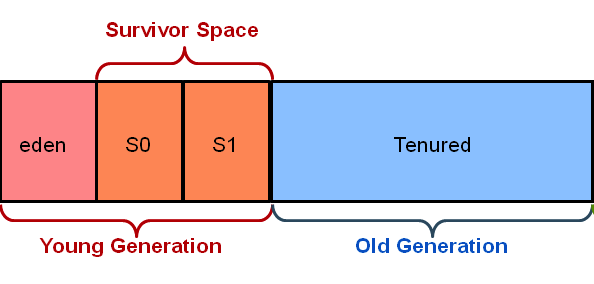
\includegraphics[width=\textwidth/2]{{figs/generational.png}}
  \caption{Generational G1 Heap Structure}
  \label{fig:generationalg1}
\end{figure*}

\subsubsection{Young GC}

Young GCs are just simple nursery GCs that only evacuate objects but not marking them.
There is no marking phase during a young GC. Instead of determining the liveness of objects
by marking, during young GCs the collector considers all objects that are not in the
to-space (i.e. the collection set) as live. The collector simply starts from the root
objects and remembered-sets to recursively evacuate live objects out of the collection-set.

\subsubsection{Mixed GC}

When the allocated memory in the heap exceeds some threshold, the generational G1 will
initiate a concurrent marking phase for a mixed GC just likes the non-generational G1.
When the to-space is exhausted during mixed GCs, G1 switches to a stop-the-world full GC.

\subsubsection{Pause time predictor for young GCs}

To meet the soft pause time goal for young GCs, the collector updates the value of \textjava{newSizeRatio}
at the end of every young GC to find a more appropriate Eden size ratio.
Then the collector can perform better in meeting the pause time goal during future young GCs.
 
\section{Shenandoah GC}
\label{sec:shenandoahgc}

Shenandoah GC is an experimental garbage collector and is originally implemented on OpenJDK.
Shenandoah GC is designed to reduce GC pause times for large heaps and tries to make the GC pause
time not proportional to the heap size.
 
When the heap occupancy reaches a threshold ratio (default is 20\%), the Shenandoah GC triggers
a concurrent GC cycle, starting from a concurrent marking phase.
The concurrent marking phase also uses the Snapshot at the Beginning algorithm,
which is similar to the G1 GC and the concurrent-marking region-based GC.
After the concurrent marking phase is a concurrent remembered-set selection phase
which is the same as the stop-the-world remembered-set selection phase
but runs concurrently, without pausing the mutators.
The third phase is the concurrent evacuation phase. Shenandoah GC uses the Brooks-style
indirection pointer (\cite{flood2016shenandoah}) to evacuate objects in to-space
concurrently. The fourth phase is the concurrent reference updating phase, which
also performs a full heap tracing, like the stop-the-world reference updating phase,
but runs concurrently, under the help of the Brooks-style indirection pointers.

By making the marking, evacuation and pointer updating phases run concurrently, Shenandoah GC performs
most of the heap scanning works concurrently, without pausing mutators. In this way,
Shenandoah GC can have very low pause times and the pause time is not proportional
to the heap size.

\subsection{Brooks indirection barrier}

% Design

The Brooks-style indirection pointer is a pointer stored in the Java object header
to record the forwarding status of a Java object (\cite{flood2016shenandoah}).
This requires the Shenandoah collector in JikesRVM to reserve an extra GC word for each
Java object. During object allocation, after a new Java object is allocated, the indirection
pointer of this Java object is initialized to point to the object itself.

During the concurrent evacuation phase, after an object is forwarded,
the collector atomically update the indirection pointer of the old copy to point to the new copy.
Mutators should always perform modification actions on the new copy of the object,
by following the indirection pointer in the object header.

By using the Brooks-style indirection pointers, the mutators can read and modify objects
(by following the indirection pointers) while the collector can also evacuate these
objects concurrently.

\subsubsection{Read Barriers}

The read operations of every object field \textjava{obj.x}, including the object
reference fields and the primitive fields, should go through the object's indirection pointer.
Figure~\ref{fig:brooksreadbarrier} shows the read barrier that is inserted before every object field read instruction.
The barrier always unconditionally extract the indirection pointer from the object header
and reads the object field value from the object that the indirection pointer points to.

\begin{figure}
  \centering
  \lstinputlisting[linewidth=\textwidth,breaklines=true]{code/brooks-read-barrier.java}
  \caption{Brooks read barrier}
  \label{fig:brooksreadbarrier}
\end{figure}

If the object is not in the collection set or is in the collection set but is not forwarded,
reading data from its original copy is safe since there is no other copies of the object
at the time the object field read happens.
If the object is forwarded, its indirection pointer is pointed to the new copy of the object.
Then by following the indirection pointer, the mutator can always read field data from the object's new copy.

\subsubsection{Write Barriers}

However, since the mutator should always meet the "write in the to space" invariant,
it is not safe for mutators to write objects just by following the indirection pointers.
If a mutator is trying to updating an object while a collector thread is also copying
this object, the write operation will only perform on the old copy and the new copy may still contain the
old data, because the indirection pointer is still pointing to the old copy when
the evacuation of this object is still in progress.

To resolve this problem, the write barrier used in Shenandoah GC is different from the
read barrier. As shown in figure~\ref{fig:brookswritebarrier}, before the mutator
performs the object field write operation on an object that is in the collection set,
the mutator first checks if the indirection pointer of the object is marked as \textjava{FORWARDED}
or \textjava{BEING_FORWARDED}. If the object is forwarded, then the mutator follows
the indirection pointer to perform the write operation on the new copy.
If the object is marked as \textjava{NOT_FORWARDED}, the mutator awaits until the object is forwarded to
get the correct indirection pointer to the new copy.
If the object is marked as not forwarded, the mutator should take the responsibility to forward this object.
Under such situation, the mutator copies this object and updates the indirection pointer,
just like the forwarding process that the collector does.

\begin{figure}
  \centering
  \lstinputlisting[linewidth=\textwidth,breaklines=true]{code/brooks-write-barrier.java}
  \caption{Brooks write barrier}
  \label{fig:brookswritebarrier}
\end{figure}

After the mutator takes the responsibility of forwarding unforwarded from-space objects,
the mutator now meets the "write in the to space" invariant. 

\subsection{Concurrent evacuation}

The evacuation phase is done mostly concurrently. Before concurrent evacuation,
the collector firstly collects and evacuate all root objects in a short stop-the-world pause.
Then during the concurrent evacuation phase, the collector linear scans each region in the
collection set to evacuate all live objects and atomically set their indirection
pointers.

JikesRVM has its own implementation of object forwarding functions, but it stores the forwarding
pointer into the status word in the object header. But by using the Brooks-style indirection
pointer, all objects should always have a valid indirection pointer stored in the header, which will override other status
information, e.g. lock and dynamic hash status. So I use a new implementation of
object forwarding functions which extends the Java header by one word and stores the indirection
pointer in this extra word.

\subsubsection{Monitor objects}

Monitor objects are handled specially in the JikesRVM implementation of the Shenandoah GC.
In JikesRVM, the JVM \textjava{monitorenter} and \textjava{monitorexit} instructions
do not triggers read barriers when locking objects, which can cause inconsistencies 
of the lock status of the object. I modified the JikesRVM's monitor lock and unlock
code to make them trigger the read barriers when necessary.

\subsection{Concurrent updating references}

Shenandoah GC also performs the update references phase concurrently.
The implementation is similar to the concurrent marking phase, but in addition to
concurrently marks objects again, the collector also updates the object reference fields
for each object and make them points the correct object.

Since the Java program is running during the concurrent reference updating phase,
unconditionally update object reference fields may cause racing problems. So instead of
unconditionally updating pointers which is used in the previous stop-the-world GCs,
I modified the procedure to perform
atomic pointer updating, as shown in figure~\ref{fig:concupdaterefs},
to avoid racing problems.

\begin{figure}
  \centering
  \lstinputlisting[linewidth=\textwidth,breaklines=true]{code/conc-update-refs.java}
  \caption{Concurrent update references}
  \label{fig:concupdaterefs}
\end{figure}

\subsubsection{Object comparisons}

Since the mutator can load an address of either the old or new copy of a same object
from the heap, simply comparing addresses of objects for the \textjava{if_acmpeq} and \textjava{if_acmpne}
instruction can cause false negatives. I implemented a new object comparison barrier,
as shown in figure~\ref{fig:objectcomparisonbarrier}, to compare object references.
Instead of simply comparing the addresses of the objects, the object comparison barrier also
compares the indirection pointers of the objects.

The comparison of the original object addresses is still required. If we only compare the
indirection pointers $a' == b'$, the GC can update the indirection pointer $b'$ to a new
address after the barrier loads $a'$ and before loads $b'$, which can still cause false
negatives if $a$ and $b$ refer to the same object.

\begin{figure}
  \centering
  \lstinputlisting[linewidth=\textwidth,breaklines=true]{code/object-comparison-barrier.java}
  \caption{Object Comparison Barrier}
  \label{fig:objectcomparisonbarrier}
\end{figure}

The object comparison barrier is implemented for both JikesRVM's baseline and optimizing compiler.

\subsubsection{Object compare and swaps}

When the Java mutator is performing object reference compare and swap operations,
the collector threads can also update the pointers contained by the slot that the CAS
is operating on. Under such situation, the CAS may fail even when there is only one mutator
thread updating the slot, since the old value is updated by the collector concurrently.

Figure~\ref{fig:objectcasbarrier} shows the object compare and swap barrier used in Shenandoah GC.
Instead of simply compare and swap with the old object, after the CAS with the old object failed,
another CAS operation is performed where the old value is the indirection pointer of the old object.
Now the overall CAS operation still succeeds if the old value is replaced with
tha address of a new copy of the same object.

\begin{figure}
  \centering
  \lstinputlisting[linewidth=\textwidth,breaklines=true]{code/object-cas-barrier.java}
  \caption{Object Reference Compare and Swap Barrier} 
  \label{fig:objectcasbarrier}
\end{figure}

\subsection{Concurrent cleanup}

The last phase of Shenandoah GC is the concurrent cleanup phase, during which the
collector concurrently visits each region in the collection set, clear their metadata
and release these regions. This phase also runs concurrently without pausing mutators.



\section{Summary}

This chapter identifies, explores and discusses the relationship of the G1 family of garbage collectors.
Then each step of of the implementation of G1 family of collectors and the involved GC algorithms
are also explained and discussed, as well as a little bit further discussion of the
pros \& cons for each structural component at an algorithmic level

However, the pros and cons of several algorithms discussed in this chapter are
all discussed based on a theoretical reasoning.
The real-world GC performance impact caused by these improvements still remains unexplored.
So to explore the real-world GC performance, in the next chapter, I will perform several performance
measurements on these collectors, and have some discussion of the evaluation results.

%%% Local Variables: 
%%% mode: latex
%%% TeX-master: "paper"
%%% End: 

% 440